\documentclass[a4paper,12pt]{scrartcl}

\newcommand{\dropsign}[1]{\smash{\llap{\raisebox{-.5\normalbaselineskip}{$#1$\hspace{2\arraycolsep}}}}}%

\usepackage[utf8]{inputenc}
\usepackage[ngerman]{babel}
\usepackage{multicol}
\usepackage{scrpage2}\pagestyle{scrheadings}
\usepackage{graphicx} 
\usepackage{pgfplots}

\ihead{Blatt 4, G2B}
\chead{Elena Noll, Sven-Hendrik Haase, E. Böhmecke}
\ohead{\today}
\pagestyle{scrheadings}
\setheadsepline{1pt}
\setcounter{secnumdepth}{0}

\begin{document}

\section{Aufgabe 14}
\section{Aufgabe 15}
\section{Aufgabe 16}
\subsection{a)}
Das "Bit stuffing" wird im HDLC-Protokoll eingesetzt um zu vermeiden das innerhab des Datenbereichs bz der Prüfsumme das Opening bzw Closing flag (Bitfolge: 01111110) auftritt.
\begin{itemize}
	\item Bitfolge: 0011111110001111101
	\item Bitfolge nach dem "Bit stuffing": 001111101100011111001
\end{itemize}
\subsection{b)}
Das Bitmuster 01111110 ist als Synchronisationszeichen geeignet, alleridngs nur solange "Bit stuffing" nach 5 aufeinanderfolgenden Einsene ingesetzt wird. Sonst könnte es vorkommen dass in den Nutzdaten zufällig die selbe Bitfolge haben wie das Synchronisationszeichen.
\subsection{c)}
Man kann mit Opening bzw. Closing Frames arbeiten. Somit weiß man wann ein Datenblock anfängt und wo er aufhört. Beim nächsten Opening Frame kann dann der jeweilige Block wieder Synchronisiert werden.
\subsection{d)}
\subsection{Ethernet}
Blocksynchronisation durch MAC-Frames (Media Access Control). Diese bestehen jeweils aus einer Präambel (7 Byte lange alternierende Bitfolge "101010...1010") gefolgt von einem Start Frame Delimeter (SFD). Die alternierende Bitfolge ermöglicht die Bitsynchronisation und das SFD (Blockanfang) die Blocksynchronisation.
\subsection{IEEE 802.11g WLANs}

\section{Aufgabe 17}
\subsection{a)}
\begin{itemize}
	\item Studen: ld(n)
	\item Knoten pro Stufe: n/2
\end{itemize}
\subsection{b)}
\begin{center}
  \makebox[\textwidth]{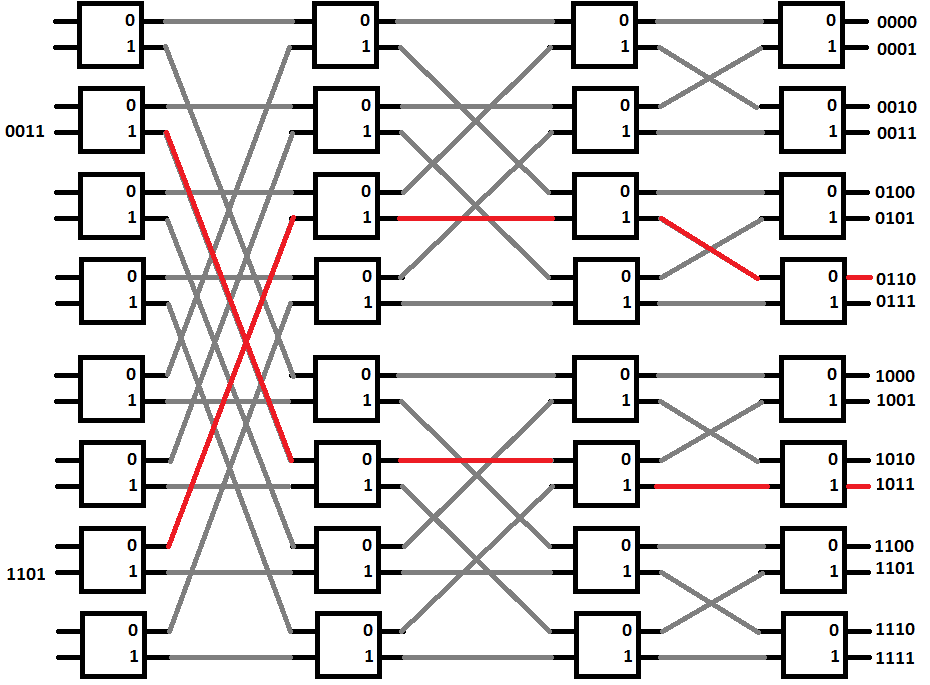
\includegraphics[width=\paperwidth]{./images/Blatt-4-Aufgabe17b}}
\end{center}
Die Zellen blockieren sich nicht auf dem Weg.
\subsection{c)}
Internet Blockierungen in einen Banyan-Netz lassen sich durch folgende Maßnahmen entschärfen:
\begin{itemize}
	\item Sort/Banyan-Netze: vorsortierung von Packeten sodass interne Blockierung vermieden wird
	\item Warteschlangen: Führt dazu dass die Leitung nur von jeweils eine Anfrage zur Zeit durchlässt.
\end{itemize}
\subsection{d)}
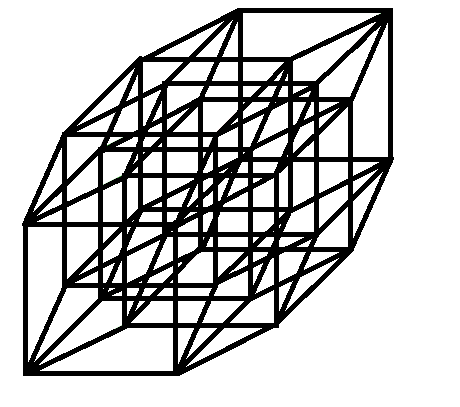
\includegraphics{./images/Blatt-4-Aufgabe17d}\\
Der 5-dimensionale Hperwürfel enthält 32 Knoten, 80 Verbindungen und 5 maximale "Hops" zwischen zwei Knoten. Da jeder Knoten 5 ausgehende Verbindungen jeweils hat, kann ein Ausfall von 5 Verbindung im ungünstigsten Fall bedeuten das 1 Knoten überhaupt nicht mehr durch eine Verbindung erreichtbar ist und somit ist auch nicht mehr sichergestellt das jeder mit jedem Knoten kommunizieren kann.
\subsection{e)}

\end{document}
